\documentclass{beamer}

% for themes, etc.
\mode<presentation>
{
%  \usetheme{Boadilla}
  \usetheme{Frankfurt}
  \usecolortheme{crane}
}

\setbeamerfont{fig_font}{size=\small}
\setbeamercovered{invisible}
\usefonttheme[onlysmall]{structurebold}
\usepackage{url}
\usepackage{times}  % fonts are up to you
\usepackage{graphicx}



% these will be used later in the title page
\title{Physics Behind the Simulation: A CS251 Report by Group 29}
\author{Shubham Jadhav \\
{\tiny 130050011}  \\
	{\tiny shubham.j@cse.iitb.ac.in}  \\
    Siddharth Bulia \\
    {\tiny 130050012}  \\
   { \tiny siddharth.bulia@cse.iitb.ac.in } \\
    Amit Malav  \\
    {\tiny 130050032}  \\
    {\tiny amit@cse.iitb.ac.in}
}
\date{October 22, 2014}

% note: do NOT include a \maketitle line; also note that this title
% material goes BEFORE the \begin{document}

% have this if you'd like a recurring outline
\AtBeginSection[]  % "Beamer, do the following at the start of every section"
{
\begin{frame}<beamer> 
\frametitle{Overview} % make a frame titled "Outline"
 % show TOC and highlight current section
\tableofcontents[currentsection]
\end{frame}
}

\begin{document}

% this prints title, author etc. info from above
\begin{frame}
\titlepage
\end{frame}

\section{Introduction}

\begin{frame}
\frametitle{Introduction}
\begin{center}
 {\bf The Mini Alarm Snoozer } 

\end{center}
\vskip 0.5in
\pause
We are creating a Rube Goldberg Machine which helps a person to snooze
the alarm. \\
\pause 
We have used many components to achieve this like Ball Elevator, Hammers,
Dominos, Inclined Planes, Pendulums, etc.
\\\pause
This report is to give an overview of our project
 % makes overlay

\end{frame}






\section{Body}

\subsection{Newton's Cradle}
\begin{frame}
\frametitle{Newton's Cradle}
{\bf Working of Newton's Cradle\cite{ref_1}}
\\\pause
Newton's Cradle work on the machanism of consecutive Collisions.
\\\pause
As all the balls are elastic, each collision simply transfer all its energy to the next ball.
\pause\\
So in final, energy is transferred to the final ball and it continues.
\pause\\
\begin{center}
{\bf Momemtum Conservation Law}
\end{center}
\begin{equation} m_1 u_{1} + m_2 u_{2} = m_1 v_{1} + m_2 v_{2}  \end{equation} 
\\
where $m_1$ ,$m_2$ are the masses and $u_1$,$u_2$,$v_1$,$v_2$ are the initial and final velocities of two bodies.
\begin{center}
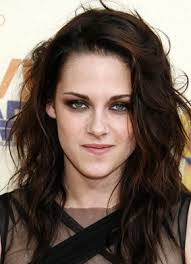
\includegraphics[width = 1.0in]{1.png}
\end{center}
\end{frame}



\subsection{Ball Elevator}
\begin{frame}
\frametitle{Ball Elevator}
{\bf Mechanism of ball Elevator}
\\
\pause
When the Newton's Cradle gives the ball to this machine, the Cross parts of this machine will coordinate with each and move the ball up.
\pause
\\The speed with which the rod will hit the ball depends on the angular velocity of rod and its length.
\pause
\\
\begin{minipage}{0.4\linewidth}
\hspace{1cm} \includegraphics[height=4cm, width = 0.5in]{2.png}
\end{minipage}%
\begin{minipage}{0.6\linewidth}
\begin{equation} v=r\omega \end{equation}
where $v$ is speed of end of rod, $r$ is the length of rod and $\omega$ is the angular velocity of rod.
\end{minipage}
\end{frame}


\subsection{Chain of Hammers}
\begin{frame}
\frametitle{Chain of Hammers}
{\bf Machanism of Chain of Hammers\cite{ref_2}}
\\\pause The ball will hit the first hammer and transfer momentum to it.
\\\pause It will swing about its revolute joint and hit the ball below and this goes on.

\pause\\
As soon as the Pulley will become free,the rock hits the alarm clock and  snooze it.
\pause\\ 
\begin{minipage}{0.4\linewidth}
\hspace{1cm}\includegraphics[width = 1.5in]{hs1.png}
\end{minipage}
\begin{minipage}{0.5\linewidth}
\begin{equation} m_1u_1=m_1v_1+m_2v_2\end{equation}
where $m_1$, $m_2$ are the masses of the ball and the hammer respectively, $u_1$ is initial linear velocity and $v_1,v_2$ are final velocities.
\end{minipage}
\end{frame}

\subsection{Dominos and The Rotating Bat}
\begin{frame}
\frametitle{Dominos and The Rotating Bat}
{\bf Machanism of Dominos and The Rotating Bat\cite{ref_3}}
\\\pause The Rotating Bat hill the ball towards the Dominos.
\\\pause The ball will hit the first dominoe and transfer momentum to the other Dominos.
\\\pause This will lead in turn to a chain reaction and at last will move the ball at the far end.

\begin{minipage}{0.4\linewidth}
%\begin{center} 
\hspace{1cm}\includegraphics[width = 1.5in]{dom.jpg}
%\end{center}
\end{minipage}
\begin{minipage}{0.4\linewidth}
%\begin{center} 
\hspace{2.5cm}\includegraphics[width = 1.5in]{rotb.jpg}
%\end{center}
\end{minipage}
%\begin{minipage}{0.5\linewidth}
%\begin{equation} m_1u_1=m_1v_1+m_2v_2\end{equation}
%where $m_1$, $m_2$ are the masses of the ball and the hammer respectively, $u_1$ is initial linear velocity and $v_1,v_2$ are final velocities.
%\end{minipage}
\end{frame}




\section{Conclusion}

\begin{frame}
\frametitle{Conclusion}

\begin{itemize}

\item This tour just scratches the surface.  
\pause

\item Through this presentation, we just described some of our elements of our project .
\pause

\item We showed the mechanism behind their working .

\end{itemize}

\end{frame}

\section{Bibliography}
\begin{frame}


\frametitle{Bibliography}
\nocite{*}
\bibliographystyle{plain}
\bibliography{bib}

\end{frame}



\end{document}

